\RequirePackage{plautopatch}
\documentclass[12pt,aspectratio=169,xcolor=dvipsnames,table,dvipdfmx, leqno]{beamer}

\usepackage{bxdpx-beamer}
\usepackage{mathtools}
\usepackage{amsmath,amsthm,amssymb,amscd}
\usepackage{ascmac}
\usepackage{physics}
\usepackage{here}
\usepackage{url}
\usepackage{bm}
\usepackage{subcaption}
\usepackage{color}
\usepackage{multirow}
\usepackage[all]{xy}
\usepackage[T1]{fontenc}
\usepackage{newtxtext} % 数式以外をTXフォントで上書き
\usepackage{ulem}
\usepackage[deluxe,uplatex]{otf} % 日本語多ウェイト化
\usepackage{algorithm}
\usepackage[noend]{algpseudocode}
\usepackage{tikz}

%Beamerの設定
\usetheme{Boadilla}

%Beamerフォント設定
\usefonttheme{professionalfonts} % Be professional!
\renewcommand{\familydefault}{\sfdefault}  % 英文をサンセリフ体に
\renewcommand{\kanjifamilydefault}{\gtdefault}  % 日本語をゴシック体に
\newcommand{\vol}{\text{vol}}
\newcommand{\round}[1]{\left\lfloor #1 \right\rceil}
\newcommand{\bhline}{\noalign{\hrule height 1.0pt}}
\DeclareMathOperator{\Pot}{Pot}
\DeclareFontFamily{U}{mathx}{}
\DeclareFontShape{U}{mathx}{m}{n}{<-> mathx10}{}
\DeclareSymbolFont{mathx}{U}{mathx}{m}{n}
\DeclareMathAccent{\widecheck}{0}{mathx}{"71}

% Babel (日本語の場合のみ・英語の場合は不要)
\uselanguage{japanese}
\languagepath{japanese}
\deftranslation[to=japanese]{Theorem}{定理}
\deftranslation[to=japanese]{Lemma}{補題}
\deftranslation[to=japanese]{Example}{例}
\deftranslation[to=japanese]{Examples}{例}
\deftranslation[to=japanese]{Definition}{定義}
\deftranslation[to=japanese]{Definitions}{定義}
\deftranslation[to=japanese]{Problem}{問題}
\deftranslation[to=japanese]{Solution}{解}
\deftranslation[to=japanese]{Fact}{事実}
\deftranslation[to=japanese]{Proof}{証明}
\def\proofname{証明}

\setbeamertemplate{theorems}[numbered]
\newtheorem{Proposition}[theorem]{命題}

%タイトル
\title[自己双対型PotBKZの提案とBKZとの比較]{ 自己双対型PotBKZ基底簡約の提案とBKZとの比較}
\author[◎~佐藤, 安田]{◎~佐藤 新\inst{1}\and 安田 雅哉\inst{1}}
\date{2025年1月29日(水)}
\institute[]{\inst{1}~立教大学}

\begin{document}
\maketitle

%=====================
\begin{frame}{研究背景}{格子暗号の安全性評価と基底簡約アルゴリズム}
%====================
\begin{itemize}
    \item \textbf{格子暗号は耐量子計算機暗号の一つ(ML-KEM, ML-DSA, Falcon)}
    \begin{itemize}
        \item 安全性はSVPやCVPなどの格子問題の求解困難性に基づく
        \item 格子暗号の安全性評価には,\uline{格子問題の求解困難性評価}が必要
    \end{itemize}
    \item \textbf{基底簡約は格子問題の求解に必須の技術}
    \begin{itemize}
        \item LLL~\cite{LLL82} $\rightsquigarrow$ 格子次元に関して多項式時間計算量
        \item BKZ~\cite{SE94}やその改良$\rightsquigarrow$ ブロックサイズに関して指数時間計算量 \\
        \begin{itemize}
            \item BKZは強力な基底簡約アルゴリズムで,安全性解析における標準ツール
            \item LLLと異なり,BKZの停止性は理論的には保証されてない
            \item 実用上,\uline{実行時間}や\uline{繰り返し(ツアー)回数}に上限を設けて\alert{強制停止} \\
            (\texttt{fplll}\cite{fpylll}内のBKZオプションとして\texttt{max\_time}や\texttt{max\_loops}がある)
        \end{itemize}
    \end{itemize}
\end{itemize}
\end{frame}

%========================
\begin{frame}{本研究の目的}{停止性を保証するBKZの変種の提案とBKZとの実験比較}
%=======================
\begin{enumerate}
    \item \textbf{停止性を保証するBKZ\cite{SE94}の変種\alert{PotBKZ}を提案}
    \begin{itemize}
        \item 基底に対して定まる\emph{ポテンシャル量}を利用
        \begin{itemize}
            \item ポテンシャル量はLLL\cite{LLL82}の多項式時間での停止性を保証する量
        \end{itemize}
        \item PotBKZでは\uline{ポテンシャル量を単調減少させる基底操作のみ}を行う\\
        % ここが一番大事
        $\implies$ 多項式回のツアー回数で停止することが保証できる
    \end{itemize}
    \item \textbf{PotBKZの様々な変種を開発+実験比較}
    \begin{itemize}
        \item 双対型や自己双対型のPotBKZまで開発
        \item BKZと実験比較:BKZとのツアー回数,出力基底の品質を比較
    \end{itemize}
\end{enumerate}
\end{frame}

% =====================================
\begin{frame}{数学的準備:格子の基礎}
% =====================================
\begin{Definition}[格子のGSOベクトルと体積]
\begin{itemize}
    \item 一次独立な$\bm{b}_1,\ldots,\bm{b}_n$の整数係数の一次結合全体
    \vspace{-8pt}
    \[
        \textstyle L=\mathcal{L}(\bm{b}_1,\ldots,\bm{b}_n)\coloneq\left\{\left.\sum_{i=1}^n{a_i\bm{b}_i}\right|a_1,\ldots,a_n\in\mathbb{Z}\right\}
    \]
    を\textbf{格子},$\{\bm{b}_1,\ldots,\bm{b}_n\}$を\textbf{基底},$n$を\textbf{次元}と呼ぶ.
    \[
        \textstyle \bm{b}_1^\star :=\bm{b}_1,~\bm{b}_i^\star :=\bm{b}_i-\sum_{j=1}^{i-1}\mu_{i,j}\bm{b}_j^\star,~\mu_{i, j} \coloneqq {\langle \bm{b}_i, \bm{b}_j^\star\rangle/\| \bm{b}_j^\star \|^2}%~(1 \!\leq\!  j \!<\! i \!\leq\! n)
%        ~(2\le i\le n)
    \]
    で定義される$\bm{b}_1^\star,\ldots,\bm{b}_n^\star$を\textbf{GSOベクトル},$\mu=(\mu_{i, j})$を\textbf{GSO係数行列}と呼ぶ.
% \end{Definition}
\item 
格子$L$の\textbf{体積}を
\[
    \textstyle\mathrm{vol}(L)=\prod_{i=1}^n\norm{\bm{b}_i^\star}
\]
と表し,\uline{これは基底にとり方によらない}
\end{itemize}
\end{Definition}
\end{frame}

% ===========================================
\begin{frame}{数学的準備:基底簡約の概要}
% ===========================================
\begin{itemize}
    \item \scalebox{1}[1]{\textbf{基底簡約}:\structure{長く平行に近い基底}を\uline{短く直交に近い基底}に変換する操作}
        \begin{itemize}
            \item 格子の基底は無数に存在
            \item 良い基底の方がSVPやCVPなどの格子問題が求解しやすい
            \item 代表的なアルゴリズム:LLL\cite{LLL82},BKZ\cite{SE94}
        \end{itemize}
\end{itemize}
\begin{figure}[htbp]
    \begin{tikzpicture}
        \draw[->] (0, 0)node [left]{
        $
        \displaystyle \left[
            \begin{array}{rrrr}
                87349 & 0 & 0 & 0 \\
                83474 & 1 & 0 & 0 \\
                98247464 & 0 & 1 & 0 \\
                847984 & 0 & 0 & 1
            \end{array}
        \right]
        $
        } -> (3, 0)node [right]{
        $
        \displaystyle \left[
            \begin{array}{rrrr}
                -8 & 8 & -1 & 3 \\
                -7 & -9 & 14 & 4 \\
                -2 & -3 & -11 & 16 \\
                8 & 6 & 12 & 17
            \end{array}
        \right]
        $
        %\draw[-] (0, 0)node[below]{基底簡約};
        };
        \node[below] at (1.5, 0){基底簡約};
        \node[below] at (-2, -1){$\mqty{\text{悪い基底}\\\structure{\text{基底のノルムが長くほぼ平行}}}$};
        \node[below] at (5, -1){$\mqty{\text{良い基底}\\\text{\alert{基底のノルムが短くほぼ直交}}}$};
    \end{tikzpicture}
\end{figure}
\end{frame}

\if 0
%===============================
\begin{frame}{ポテンシャル量(1/2):ポテンシャル量の定義}
%===============================
\begin{Definition}[ポテンシャル量]
    \begin{itemize}
        \item $\{\bm{b}_1,\ldots,\bm{b}_n\}$:$n$次元格子$L$の基底
        \item $\bm{b}_1^\star,\ldots,\bm{b}_n^\star$:$\bm{b}_1,\ldots,\bm{b}_n$のGSOベクトル
        \item $L$の部分格子$L_i\coloneqq\mathcal{L}(\bm{b}_1,\ldots,\bm{b}_i)$に対して
    \end{itemize}
    \[
        \mathrm{Pot}(\{\bm{b}_1,\ldots,\bm{b}_n\}) \coloneqq \prod_{i=1}^n \mathrm{vol}(L_i)^2 = \prod_{k=1}^{n} \| \bm{b}_k^\star \|^{2(n-k+1)} > 0
    \]
    を$\qty{\bm{b}_1,\ldots,\bm{b}_n}$の\textbf{ポテンシャル量}と呼ぶ.
\end{Definition}
\end{frame}
\fi 

% =================================================
\begin{frame}{ポテンシャル量とLLLアルゴリズム}
% =================================================
\uline{基底$\{\bm{b}_1,\ldots,\bm{b}_n\}$の\alert{ポテンシャル量}}
% \vspace{-8pt}
\[\textstyle\mathrm{Pot}(\{\bm{b}_1,\ldots,\bm{b}_n\}) \coloneqq \prod_{k=1}^{n} \| \bm{b}_k^\star \|^{2(n-k+1)} > 0\]
% \footnotesize
%\begin{figure}[tbp]
\vspace{-14pt}
\begin{minipage}[b]{0.45\columnwidth}
    \uline{LLLアルゴリズム}\cite{LLL82}
    \begin{itemize}
        \item 次の条件を満たす基底を見つける
        \begin{enumerate}
            \item
            % サイズ簡約条件 
            $\abs{\mu_{i, j}}\le 1/2$
            \item
            % Lov\'asz条件 
            $\delta\cdot \norm{\bm{b}_{k-1}^\star}^2\le\norm{\pi_{k-1}(\bm{b}_k)}^2$
        \end{enumerate}
        \item 特に,条件2を満たさない$(\bm{b}_k, \bm{b}_{k+1})$を交換(Step 7)
        \begin{itemize}
            \item \uline{ポテンシャルが$\delta$倍ずつ減少} \\
            $\implies$ \alert{\textbf{多項式時間で停止}}
        \end{itemize}
    \end{itemize}
    \mbox{}\\
    \mbox{}\\
    \mbox{}\\
    \mbox{}\\
\end{minipage}
\hspace{0.03\columnwidth} % ここで隙間作成
\begin{minipage}[b]{0.45\columnwidth}
    \begin{algorithm}[H]
    \footnotesize
        \begin{algorithmic}[1]
            \caption{\footnotesize LLL基底簡約アルゴリズム\cite{LLL82}}
            \label{alg_LLL}
            \Require{格子$L$の基底$\{\bm{b}_1,\ldots,\bm{b}_n\}$}
            \Statex 定数$1/4<\delta<1$
            \Ensure{$\delta$に関してLLL簡約された基底}
            \State $k \gets 2$
            \While{$k\le n$}
                \State 基底をサイズ簡約\cite{Hermite1850}
                \If{条件$2$を満たす}
                    \State $k\gets k+1$
                \Else
                    \State swap$(\bm{b}_k, \bm{b}_{k+1})$
                    % /*~基底のポテンシャル量が$\delta$倍される*/
                    \State $k\gets\max\{k-1, 2\}$
                \EndIf
            \EndWhile
        \end{algorithmic}
    \end{algorithm}
    \mbox{}\\
\end{minipage}
%\end{figure}
\end{frame}

% ========================================
\begin{frame}{DeepLLLアルゴリズムとPotLLLアルゴリズム}
% ========================================
\uline{基底に対する\alert{deep-inserion}という操作}
\[
\sigma_{k, \ell}(\qty{\bm{b}_1,\ldots,\bm{b}_n})=\{\ldots, \bm{b}_{k - 1}, \bm{b}_\ell, \bm{b}_{k}, \ldots, \bm{b}_{\ell-1}, \bm{b}_{\ell+1}\ldots\}
\]
\begin{minipage}[b]{0.45\columnwidth}
    \uline{DeepLLLアルゴリズム}\cite{SE94}
    \begin{itemize}
        \item 次の条件を満たす基底を見つける
        \begin{enumerate}
            \item $\abs{\mu_{i, j}}\le 1/2$
            \item $\delta\cdot \norm{\bm{b}_i^\star}^2\le\norm{\pi_{i}(\bm{b}_k)}^2$ 
        \end{enumerate}
        \item 条件2を満たさない基底をdeep-insertionで入れ替え
        \begin{itemize}
            \item \scalebox{0.9}[1]{ポテンシャルは\structure{増えたり減ったり}}\\
            $\implies$ \structure{\textbf{指数時間}}
        \end{itemize}
    \end{itemize}
    \mbox{}\\
\end{minipage}
\begin{minipage}[b]{0.45\columnwidth}
    \uline{PotLLLアルゴリズム}\cite{FSW14}
    \begin{itemize}
        \item 次の条件を満たす基底を見つける
        \begin{enumerate}
            \item $\abs{\mu_{i, j}}\le 1/2$
            \item $\delta\cdot \mathrm{Pot}(\bm{B})\le\mathrm{Pot}(\sigma_{k, \ell}(\bm{B}))$\label{condition:polll-2}
        \end{enumerate}
        \item 条件\ref{condition:polll-2}を満たさない基底をdeep-insertionで入れ替え
        \begin{itemize}
            \item \mbox{}\\
            \vspace{-13pt}
            \scalebox{0.9}[1]{$\mathrm{Pot}(\bm{B})$を下げるdeep-insertionのみ}
            \item ポテンシャルが単調減少\\
            $\implies$\alert{\textbf{多項式時間で停止}}
        \end{itemize}
    \end{itemize}
    \mbox{}
\end{minipage}
\end{frame}

\if 0
% ======================================
\begin{frame}[fragile]{PotLLLの概要}
% ======================================
\footnotesize
\begin{minipage}[b]{0.45\columnwidth}
   \begin{Definition}[PotLLL簡約]
        \begin{itemize}
            \item $\bm{B}$:$n$次元格子の基底
            \item $\mu_{i, j}$:$\bm{B}$のGSO係数
            \item $\delta$:簡約変数
        \end{itemize}
        \begin{enumerate}
            \item $1\le{}^\forall j<{}^\forall i\le n,~ \abs{\mu_{i, j}}\le\frac{1}{2}$

            \item $1\le{}^\forall k<{}^\forall \ell\le n,~\delta\cdot \text{Pot}(\bm{B})\le\text{Pot}(\sigma_{k, \ell}(\bm{B}))$
        \end{enumerate}
    \end{Definition}
    \begin{itemize}
        \item 基底のポテンシャル量を下げる
        \begin{itemize}
            \item \textbf{格子次元に関して多項式時間}
        \end{itemize}
    \end{itemize}
\end{minipage}
\hspace{0.03\columnwidth}
\begin{minipage}[b]{0.45\columnwidth}
    \begin{algorithm}[H]
    \footnotesize
        \begin{algorithmic}[1]
            \caption{\footnotesize PotLLL基底簡約アルゴリズム\cite{FSW14}}
            \label{alg_PotLLL}
            \Require{$n$次元格子の基底$\{\bm{b}_1,\ldots,\bm{b}_n\}$,簡約変数$\frac{1}{4}<\delta<1$}
            \Ensure{$\delta$に関してPotLLL簡約された基底}
            \State $\bm{B}\gets \texttt{LLL}(\bm{B}, \delta)$
            \State $\ell \gets 1$
            \While{$\ell\le n$}
                \State $\bm{B}$をサイズ簡約
                \State $P_\text{min}\gets \min_{1\le j\le \ell}\frac{\Pot(\sigma_{j, \ell}(\bm{B}))}{\Pot(\bm{B})}$
                \If{$\delta>P_{\min}$}
                    \State $\bm{B}\gets \sigma_{k, \ell}(\bm{B})$
                    \State $\ell\gets k$
                \Else
                    \State $\ell\gets\ell +1$
                \EndIf
            \EndWhile
        \end{algorithmic}
    \end{algorithm}
\end{minipage}
\end{frame}
\fi

% ===================================
\begin{frame}{PotENUM:PotLLLの一般化}
% ===================================
\begin{itemize}
\item $\mathrm{Pot}(\bm{B})$を減少させる格子ベクトル$\bm{v} = \sum_{i=j}^m v_i \bm{b}_i~(v_m = 1)$の数え上げ
    \begin{itemize}
    \item $\bm{C} = \{\ldots, \bm{b}_{j-1}, \bm{v}, \bm{b}_j,\ldots, \widecheck{\bm{b}_m}, \ldots \}$:$j$番目に$\bm{v}$を挿入+$\bm{b}_m$を除去
    % \item $\bm{C}$: 一次従属性を除去して得られる新しい$L$の基底
    \item $\mathrm{Pot}(\bm{C}) < \mathrm{Pot}(\bm{B})$ \\
    (cf., PotLLL\cite{FSW14}ではdeep-insertion $\sigma_{j, m}$で得られる基底に限定)
    \end{itemize}
\item 従来のENUM\cite{GNR10}とPotENUMの比較($D_i\coloneq \norm{\pi_i(\bm{v})},~B_i\coloneq\norm{\bm{b}_i^\star}$)
%\item 基底のポテンシャルが必ず\uline{減少する}ベクトルを探索するアルゴリズム
%\begin{itemize}
%    \item[PotLLL] deep-insertionでポテンシャル量が減少する基底を探す
%    \item[PotENUM] 基底への挿入でポテンシャル量が減少するベクトルを探索する\\
%    \quad $\implies$\uline{基底の入れ替えだけでは見つからない基底も見つけられる}
%\end{itemize}
\end{itemize}
\begin{figure}[htbp]
    \begin{table}[]
        \centering
        \begin{tabular}{c|c|c}
             & ENUM\cite{GNR10} & PotENUM\\
            \bhline
            $\bm{v}$の条件 & $D_j<B_j$ &\alert{$\displaystyle D_j^j \prod_{i=j+1}^{m-1}D_i^2<\delta\prod_{i=1}^{m-1}B_i$}\\
            \hline
            探索方法 & $D_j<R^2$ & $\alert{D_j<R_j^2},~R_j^2=\qty(\dfrac{\delta B_1\cdots B_{m-1}}{D_{k+1}\cdots D_{m-1}})^{1/j}$\\
            \hline
            挿入による効果 & $\| \bm{b}_j^\star \|$を減少 & \alert{$\mathrm{Pot}(\bm{B})$を減少} 
%             & 数え上げる格子ベクトル$\bm{v}$の条件 & $\bm{v}$の挿入による効果 \\
%            \bhline
%            ENUM &  $\displaystyle\norm{\bm{b}_j^\star}^2>\norm{\pi_j(\bm{v})}^2$ & $\| \bm{b}_j^\star \|$を減少\\
%            \hline
%            PotENUM &  & \alert{$\mathrm{Pot}(\bm{B})$を減少}
        \end{tabular}
        % \caption{PotENUMとENUMの違い}
        \label{tab:my_label}
    \end{table}

%    \begin{tikzpicture}
%        \draw (0, 6) node [above]{ENUM} -- (0, 4) node [below, align=center]{
%            $\norm{\bm{b}_j^\star}>\norm{\pi_j(\bm{v})}$なるベクトルを\\基底の$j$番目に挿入
%        };
%        \draw[->] (0, 2.7) -> (0, 0.7) node [below]{$k$番目のGSOベクトルを短く};
%        \draw (8, 6) node [above]{\alert{PotENUM}} -- (8, 4) node [below, align=center]{\alert{$D_k^{k} \cdot D_{k+1} \cdots D_{m-1} < \delta B_1 \cdots B_{m-1}$}\\なるベクトルを$j$番目に挿入};
%        \draw[->] (8, 2.7) -> (8, 0.7) node [below]{\textbf{\alert{基底のポテンシャル量}を小さく}};
 %   \end{tikzpicture}
\end{figure}
\end{frame}

% ==============================================
\begin{frame}{PotBKZ(1/2):BKZとの構成の差異}
% ==============================================
\begin{figure}[htbp]
    \begin{tikzpicture}
        \draw (0,0) node [below]{LLL\cite{LLL82}} -- (0,1.5) -- (4,1.5) -- (4,0) node [below]{ENUM\cite{GNR10}};
        \draw (2,1.5) -- (2,3) node [above]{BKZ\cite{SE94}};
        \draw (7,0) node [below]{PotLLL\cite{FSW14}} -- (7,1.5) -- (11,1.5) -- (11,0) node [below]{\alert{$\mqty{\text{PotENUM}\\\textbf{今回開発}}$}};
        \draw (9,1.5) -- (9,3) node [above]{\alert{$\mqty{\textbf{今回開発}\\\text{PotBKZ}}$}};
    \end{tikzpicture}
\end{figure}
\begin{itemize}
    \item PotBKZではBKZのLLLをPotLLLに,ENUMをPotENUMに置き換え
    \item PotLLLとPotENUMはどちらもポテンシャルを単調減少
    \begin{itemize}
        \item PotENUMが呼ばれる回数(ツアー回数)は\alert{\textbf{格子次元に関して多項式的}}
    \end{itemize}
%    \item[$\rightsquigarrow$] PotENUMが呼ばれる回数(ツアー回数)は\alert{\textbf{格子次元に関して多項式時間計算量}}
    %\item[$\rightsquigarrow$] BKZは\structure{格子次元に関して指数的で\uline{停止性は保証されない}}
\end{itemize}
\end{frame}

% ==========================================
\begin{frame}[fragile]{PotBKZ(2/2):アルゴリズムの概要}
% ==========================================
\begin{algorithm}[H]
    \footnotesize
    \begin{algorithmic}[1]
        \caption{\footnotesize PotBKZ基底簡約アルゴリズム}
        \Require{$n$次元格子の基底$\{\bm{b}_1,\ldots,\bm{b}_n\}$,簡約変数$1/4<\delta<1$}
        \Ensure{簡約された基底$\{\bm{b}_1,\ldots,\bm{b}_n\}$}
        \State $\{\bm{b}_1,\ldots,\bm{b}_n\}\gets \alert{\texttt{PotLLL}(\{\bm{b}_1,\ldots,\bm{b}_n\}, \delta)}$~/*~BKZ\cite{SE94}ではLLL\cite{LLL82}を利用*/
        \State $z \gets 0$
        \While{$z<n-1$}
            \State $j \gets (j \bmod{n-1}) + 1; k \gets \min(j + \beta-1, n)$
            \State $\bm{v}\gets \alert{\texttt{PotENUM}(\pi_j(\bm{b}_j), \dots, \pi_j(\bm{b}_k))}$~/*~BKZではENUM\cite{GNR10}で最短ベクトルを探索*/
            \If{no~solution}
                \State $z\gets z+1$
            \Else
                \State $\{\bm{b}_1,\ldots,\bm{b}_n\}\gets \texttt{MLLL}(\{\ldots,\bm{b}_j, \bm{v},\bm{b}_{j+1},\ldots\}, \delta)$~/*~MLLL\cite{SE94}で一次独立性を除く*/
                \State $\{\bm{b}_1,\ldots,\bm{b}_n\}\gets \alert{\texttt{PotLLL}(\{\bm{b}_1,\ldots,\bm{b}_n\}, \delta)}$
                \State $z\gets 0$
            \EndIf
        \EndWhile
    \end{algorithmic}
\end{algorithm}
\end{frame}

\if 0
% ===============================================
\begin{frame}{双対型PotENUM}
% ===============================================
\begin{itemize}
    \item \textbf{ポテンシャル量をより下げるため\alert{自己双対型}を開発}
    \begin{itemize}
        %\item 双対基底に対してPotBKZを行う
        \item \uline{双対基底に挿入する}ことでポテンシャル量を下げる必要
        \item \textbf{\alert{双対型PotENUMアルゴリズム}}を開発
    \end{itemize}
    \item \textbf{双対基底に対してPotBKZを行う手順}
    \begin{itemize}
        \item 本来,双対基底を求めるには\structure{\textbf{逆行列計算が必要}}
        %\begin{itemize}
            \item しかし
            \begin{align*}
                \frac{1}{\norm{\bm{b}^\star_1}^2\cdots \norm{\bm{b}^\star_{m-1}}^2}<\norm{\tau_1(\bm{v})}^2\cdots \norm{\tau_{m-3}(\bm{v})}^2\norm{\tau_{m-2}(\bm{v})}^{4}
            \end{align*}
            なるベクトルの双対基底への挿入でポテンシャル量を下げられる
            \item \alert{\textbf{逆行列を計算する必要がなくなる}}
        %\end{itemize}
        \item 双対型PotENUMは\textbf{基底の情報のみから}双対基底のポテンシャル量を増加
    \end{itemize}
\end{itemize}
\end{frame}

% ===============================================
\begin{frame}[fragile]{自己双対型PotBKZの概要:双対型PotBKZ}
% ===============================================
\begin{minipage}[b]{0.45\columnwidth}
    \begin{algorithm}[H]
    \footnotesize
        \begin{algorithmic}[1]
            \caption{\footnotesize primal~part}
            \State $\bm{v}\gets \texttt{PotENUM}(\pi_j(\bm{b}_j), \dots, \pi_j(\bm{b}_k))$
            \If{no~solution}
                \State 次のステップへ
            \Else
                \State $\bm{v}$を基底の$j$番目に挿入
                %\State $\{\bm{b}_1,\ldots,\bm{b}_n\}\gets \texttt{MLLL}(\{\ldots,\bm{b}_j, \bm{v},\bm{b}_{j+1},\ldots\}, \delta)$~/*~MLLL\cite{SE94}で一次独立性を除く*/
                \State $\alert{\texttt{DualPotLLL}(\{\bm{b}_1,\ldots,\bm{b}_n\}, \delta)}$
                %\State $z\gets 0$
            \EndIf
        \end{algorithmic}
    \end{algorithm}
\end{minipage}
\begin{minipage}[b]{0.45\columnwidth}
\begin{algorithm}[H]
\footnotesize
    \begin{algorithmic}[1]
        \caption{\footnotesize dual~part}
        %\State $z \gets 0$
        %\State $j \gets (j \bmod{n-1}) + 1; k \gets \min(j + \beta-1, n)$
        \State $\bm{v}\gets \alert{\texttt{DualPotENUM}(\pi_j(\bm{b}_j), \dots, \pi_j(\bm{b}_k))}$
        \If{no~solution}
            \State 次のステップへ
        \Else
            \State $\bm{v}$を双対基底の$j$番目に挿入\cite{MW16}
            % \State $\{\bm{b}_1,\ldots,\bm{b}_n\}\gets \texttt{MLLL}(\{\ldots,\bm{b}_j, \bm{v},\bm{b}_{j+1},\ldots\}, \delta)$~/*~MLLL\cite{SE94}で一次独立性を除く*/
            \State $\alert{\texttt{PotLLL}(\{\bm{b}_1,\ldots,\bm{b}_n\}, \delta)}$
            %\State $z\gets 0$
        \EndIf
    \end{algorithmic}
\end{algorithm}
\end{minipage}
\begin{itemize}
    \item 自己双対型PotBKZはprimal~partとdual~partを交互に行う
    \begin{itemize}
        \item どちらかが連続$n-1$回繰り返されたら停止
    \end{itemize}
\end{itemize}
\end{frame}
\fi

% ==============================================
\begin{frame}{自己双対型PotBKZ:自己双対型BKZとの構成の差異}
% ==============================================
\begin{figure}[htbp]
    \begin{tikzpicture}
        \draw (0,0) node [below]{BKZ\cite{SE94}} -- (0,1) -- (4,1) -- (4,0) node [below]{双対型BKZ\cite{MW16}};
        \draw (2,1) -- (2,2) node [above]{自己双対型BKZ\cite{MW16}};
        \draw (7,0) node [below]{PotBKZ} -- (7,1) -- (11,1) -- (11,0) node [below]{\alert{$\mqty{\text{双対型PotBKZ}\\\textbf{今回開発}}$}};
        \draw (9,1) -- (9,2) node [above]{$\alert{\mqty{\textbf{今回開発}\\\text{自己双対型PotBKZ}}}$};
    \end{tikzpicture}
\end{figure}
\vspace{-10pt}
\begin{itemize}
    \item 自己双対型PotBKZはPotBKZとその双対型を\textbf{交互に呼び出す}
    \item 双対型PotBKZを開発
    \begin{itemize}
        \item 双対基底を求めるには\structure{\textbf{逆行列計算}が必要}
        \item \scalebox{0.95}[1]{双対型PotENUM$\rightsquigarrow$\uline{双対基底への挿入}でポテンシャルが減少するベクトルの数え上げ}
        \item \textbf{逆行列計算が\alert{不要}}
    \end{itemize}
%    \item PotLLLとPotENUMはどちらもポテンシャルを単調減少
%    \begin{itemize}
%        \item PotENUMが呼ばれる回数(ツアー回数)は\alert{\textbf{格子次元に関して多項式的}}
%    \end{itemize}
%    \item[$\rightsquigarrow$] PotENUMが呼ばれる回数(ツアー回数)は\alert{\textbf{格子次元に関して多項式時間計算量}}
    %\item[$\rightsquigarrow$] BKZは\structure{格子次元に関して指数的で\uline{停止性は保証されない}}
\end{itemize}
\end{frame}

%====================================
\begin{frame}{実験結果(1/3):実装方法と実験方法}
%====================================
\begin{itemize}
    \item \textbf{実装方法}
    \begin{itemize}
        \item 実装は総て\texttt{C++}言語で\texttt{NTL}ライブラリ\cite{NTL}と\texttt{Eigen}ライブラリ\cite{Eigen}を使用
        \item \texttt{g++}でコンパイル
        \item コンパイルオプションは\texttt{-O3 -mtune=native -march=native -mfpmath=both}
        \item 基底は\texttt{long}型,GSO情報は\texttt{long double}型を使用
    \end{itemize}
    \item \textbf{実験方法}
    \begin{itemize}
        \item SVP-challenge\cite{SVP}のシード0~9で実行
        \item \textbf{ツアー回数},\textbf{ポテンシャル量の対数値},\textbf{GSAスロープの傾き}の平均をとる
        \begin{itemize}
            \item GSAスロープの傾きは良い基底を判断する指標の一つ(小さい方が良い)
        \end{itemize}
    \end{itemize}
\end{itemize}
\end{frame}

%========================================================
\begin{frame}{実験結果(2/3):100次元のポテンシャル量の変化}
%========================================================
\begin{figure}[t]
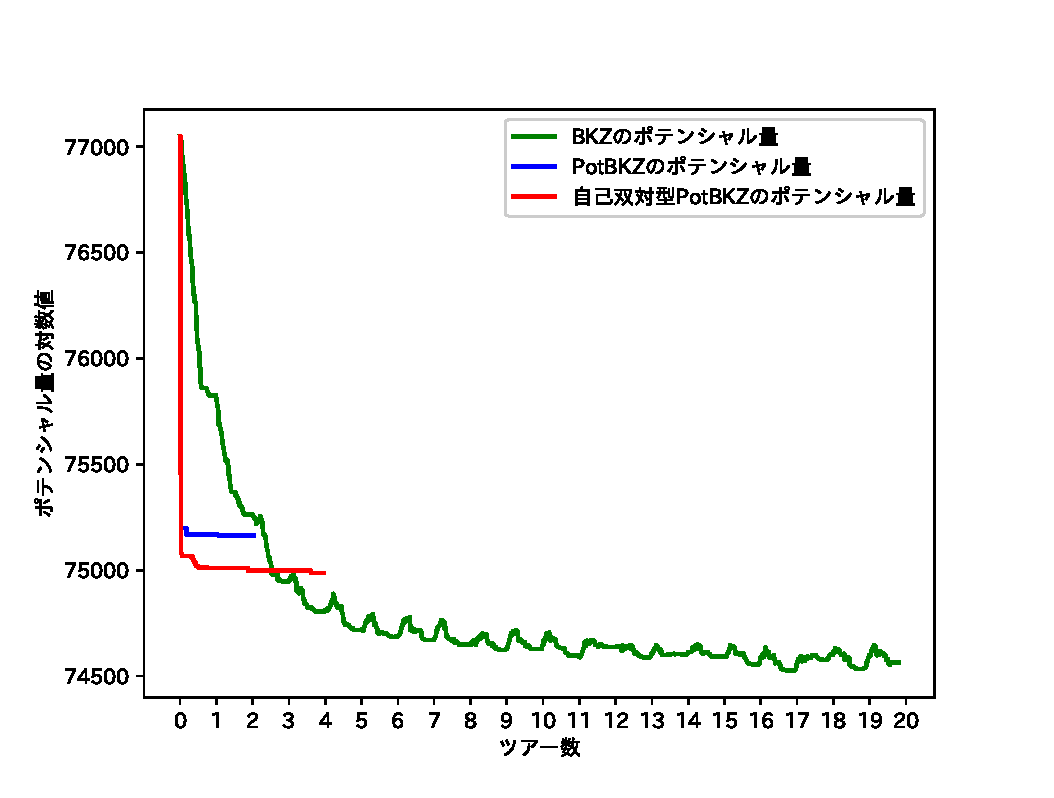
\includegraphics[height = 150pt]{100_compare_potential.eps}
\end{figure}
\begin{itemize}
    \footnotesize
    \item \textbf{PotBKZ}は1ツアー目で一気にポテンシャルが低くなり,その後\alert{2ツアーで\textbf{停止}}
    \item \textbf{自己双対型PotBKZ}も同様の挙動を取り\alert{4ツアーで\textbf{停止}}
    \begin{itemize}
        \item PotBKZより\alert{小さいポテンシャル量をとる}
    \end{itemize}
    \item 一方,\textbf{BKZ}\cite{SE94}は緩やかに減少し,その後\structure{7ツアー目頃から\textbf{停滞}を続ける}
\end{itemize}
\end{frame}

%=========================================================
\begin{frame}{実験結果(3/3):}
%=========================================================
\begin{itemize}
    \item \textbf{実験結果}
    \begin{itemize}
        \item Intel Core i7-1355U @ 1.70 GHz上で実験
        \item ブロックサイズは$\beta=40$を選択
        \item PotBKZは\alert{約2回程度のツアー回数}で停止
        \item 自己双対型PotBKZも\alert{約5回程度のツアー回数で停止}
        \begin{itemize}
            \item PotBKZよりも\textbf{\alert{低い}GSAスロープの傾きとポテンシャル量の対数値の比をとる}
        \end{itemize}
        \item 一方, BKZ\cite{SE94}と比較すると
        \structure{高く,\textbf{十分に下げられていない}}
    \end{itemize}
\end{itemize}
\vspace{-1.5mm}
\begin{table}[t]
    \footnotesize
    \centering
%      \caption{ブロックサイズ$\beta=40$のBKZ,PotBKZ,及び自己双対型PotBKZのツアー数,$\log\Pot{(\bm{B})}$,及びGSAスロープの傾きの負値の平均値についての実験結果}
    \label{table:1}
    \begin{tabular}{c||c|c|c|c|c|c|c|c|c}
        \bhline
        \multirow{2}{*}{格子}  & 
        \multicolumn{3}{c|}{BKZ\cite{SE94}} &
        \multicolumn{3}{c|}{PotBKZ} & \multicolumn{3}{c}{自己双対型PotBKZ} \\
        \cline{2-10}
        \multirow{2}{*}{階数} & ツアー & $\log \Pot$ & \multirow{2}{*}{$-\rho$} & 
        ツアー & $\log \Pot$ & \multirow{2}{*}{$- \rho$} & ツアー & $\log \Pot$ & \multirow{2}{*}{$- \rho$} \\
        & 回数 & の比 & & 回数 & の比 & & 回数 & の比 &\\
        \bhline
        100 & $\ge 20$ & 0.9668 & 0.0553 & 1.9 & 0.9735 & 0.0615 & 4.8 & 0.9714 & 0.0595 \\
        110 & $\ge 20$ & 0.9658 & 0.0561 & 1.9 & 0.9722 & 0.0617 & 5.2 & 0.9697 & 0.0594 \\
        120 & \structure{$\ge 20$} & 0.9616 & 0.0558 & \alert{1.7} & 0.9685 & 0.0612 & \alert{5.9} & 0.9665 & 0.0597 \\
        \bhline
    \end{tabular}
\end{table}
\end{frame}

%==============
\section{まとめ}
%==============
\begin{frame}{まとめ}
\begin{itemize}
    \item \textbf{PotBKZと自己双対型PotBKZの開発と実験}
    \begin{itemize}
        \item ポテンシャルの単調減少により停止性の保証されたBKZ\cite{SE94}の変種
        \item 基底への挿入でポテンシャルが減少するベクトルを数え上げるPotENUMを開発
        \item その双対版,自己双対版を開発
        \item 120次元格子での実験結果\\
        \begin{itemize}
            \item[$\rightsquigarrow$] \alert{PotBKZは\textbf{2ツアー程度},自己双対型PotBKZは\textbf{5ツアー程度}で停止}
            \item[$\rightsquigarrow$] 一方BKZは\structure{\textbf{20ツアー以上を要する}}
        \end{itemize}
    \end{itemize}
    \item \textbf{今回の実験結果から得られた知見}
    \begin{itemize}
        \item PotBKZや自己双対型PotBKZはBKZほど\structure{ポテンシャルを下げれない}
        \begin{itemize}
            \item より大きなブロックサイズを試せば\uline{BKZ程度の品質が出せると期待}
            \item より大きなブロックサイズの利用のため,\textbf{枝切り}や\textbf{篩}の適用をしたい
        \end{itemize}
    \end{itemize}
\end{itemize}
\end{frame}

\begin{frame}{PotBKZとその変種の公開ソースコード}
\begin{itemize}
    \item 本研究の成果となるソースコードを\texttt{GitHub}にて公開\\
    \url{https://github.com/satoshin-des/self-dual-PotBKZ}
    \item ファイル構成\\
    ┣━━\texttt{src}\\
    ┃~~~~~~~┃\\
    ┃~~~~~~~┗━━各種ソース(\texttt{SelfDualPotBKZ.h},\texttt{PotBKZ.h}など)\\
    ┣━━\texttt{svp\_challenge\_list}\\
    ┃~~~~~~~┃\\
    ┃~~~~~~~┗━━テストケースとして\texttt{svp~challenge}\cite{SVP}の基底(LLL済)\\
    ┣━━\texttt{libSDPotBKZ.so}\\
    ┃~~~~~~~~~~$\rightsquigarrow$C++ファイルをコンパイルした共有ライブラリ\\
    ┗━━\texttt{excample.py}\\
    \quad~~~~~~~~~~$\rightsquigarrow$\texttt{libSDPotBKZ.so}を\texttt{python}で動かすテストコード
\end{itemize}
\end{frame}

\section{参考文献}
\begin{frame}[allowframebreaks]{参考文献}
\beamertemplatetextbibitems
\bibliographystyle{plain}
\bibliography{ref}
\end{frame}
\end{document}